\icode[magenta]{N23X-MM-CA-L4-261014-001}
\nceeID{2023湖南}{15}
如图，质量为\(M\)的匀质凹槽放在光滑水平地面上，凹槽内有一个半椭圆形的光滑轨道，椭圆的半长轴和半短轴分别为\(a\)和\(b\)，长轴水平，短轴竖直，质量为\(m\)的小球，初始时刻从椭圆轨道长轴的右端点由静止开始下滑，以初始时刻椭圆中心的位置为坐标原点，在竖直平面内建立固定于地面的直角坐标系\(xOy\)，椭圆长轴位于\(x\)轴上。整个过程凹槽不翻转，重力加速度为\(g\)。
\begin{enumerate}
	\item 小球第一次运动到轨道最低点时，求凹槽的速度大小以及凹槽相对于初始时刻运动的距离；
	\item 在平面直角坐标系\(xOy\)中，求出小球运动的轨迹方程；
	\item 若\(\frac{M}{m} = \frac{b}{a - b}\)，求小球下降\(h = \frac{b}{2}\)高度时，小球相对于地面的速度大小(结果用\(a\)、\(b\)及\(g\)表示)。
\end{enumerate}

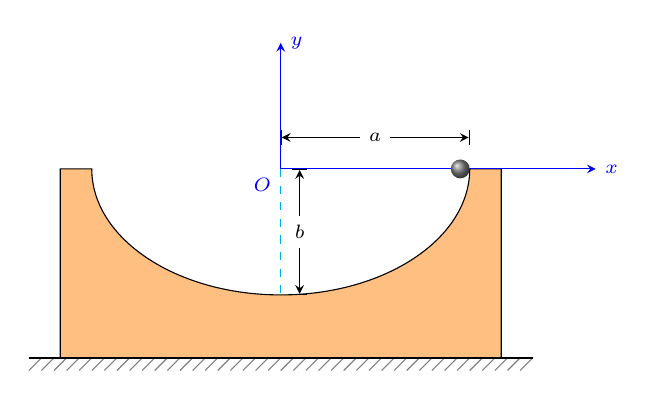
\begin{tikzpicture}[>=stealth,scale=.8,font=\scriptsize]
    \draw[fill=orange!50] (3,0) arc(0:-180:3 and 2)--(-3.5,0)--(-3.5,-3)--(3.5,-3)--(3.5,0)--(3,0);
	\draw[->,blue] (0,0)node[below left]{\(O\)}--(5,0)node[right]{\(x\)};
	\draw[->,blue] (0,0)--(0,2)node[right]{\(y\)};
	\shade[ball color=gray] (2.85,0) circle(.15);
	\draw[|<->|] (0,.5)--node[fill=white]{\(a\)}(3,.5);
	\draw[dashed,cyan] (0,0)--(0,-2);
	\draw[|<->|] (.3,0)--node[fill=white]{\(b\)}(.3,-2);
	\foreach \x in {-4,-3.8,...,3.8}
		\draw[gray] (\x,-3.2)--++(.2,.2);
	\draw[thick] (-4,-3)--(4,-3);
\end{tikzpicture}
\begin{answer}
	（1）\(v_2 = \sqrt{\frac{2m^2gb}{M^2 + Mm}}\)\quad \(x_2 = \frac{m}{M + m}a\)（2）\(\frac{[x(M + m) - ma]^2}{M^2a^2} + \frac{y^2}{b} = 1\)（3）\(2b \sqrt{\frac{g}{a + 3b}}\)
\end{answer}